\documentclass[master=eelt, english]{kulemt}

\setup{
title={Implementation and Evaluation of Zero-Knowledge Proofs of Knowledge},
author={Boran Car},
promotor={Bart Preneel \and Ingrid Verbauwhede},
assessor={Claudia Diaz \and Francky Catthoor},
assistant={Josep Balasch \and Alfredo Rial}
}

\usepackage[pdfusetitle,colorlinks,plainpages=false]{hyperref}
\usepackage{biblatex}
\usepackage{tikz}
\usepackage{tikz-qtree}
\usepackage[caption=false]{subfig}
\usepackage{tabularx}
\usepackage{color}
\usepackage{amsmath}
\usepackage{listings}
\usepackage{amsfonts}
\usepackage{amsthm}
\usepackage{algpseudocode}
\usepackage{algorithm}

\theoremstyle{definition}
\newtheorem{defn}{Definition}
\newtheorem{thm}{Theorem}

\definecolor{dkgreen}{rgb}{0,0.6,0}
\definecolor{gray}{rgb}{0.5,0.5,0.5}
\definecolor{mauve}{rgb}{0.58,0,0.82}

\lstdefinelanguage{PIL}{
morekeywords={ExecutionOrder, Common, Def, Void, Prime, Z, Int},
otherkeywords={Zmod+, Zmod*},
morecomment=[l]{//},
morecomment=[s]{/*}{*/}
}

\lstset{
language=PIL,
basicstyle=\footnotesize,
commentstyle=\color{dkgreen},
keywordstyle=\bfseries,
frame=single,
breaklines=true,
breakatwhitespace=false
}

\usetikzlibrary{backgrounds,calc,shapes,shadows,arrows,chains,trees,fit,positioning}

\tikzstyle{language}=[rectangle,draw=black,thin,inner sep=3pt, align=center]

\tikzstyle{compiler}=[rectangle,rounded corners,draw=black,thin,inner
sep=3pt, align=center]

\tikzstyle{added}=[fill=gray]

\addbibresource{references}

\begin{document}

\begin{preface}

\end{preface}

\tableofcontents*

\begin{abstract}

\end{abstract}

\listoffigures

\listoftables

\mainmatter

\chapter{Introduction}

\section{Zero Knowledge Proofs of Knowledge}

Today's state-of-the-art cryptosystems are based on the following hard
problems:
\begin{itemize}
\item Discrete Logarithm Problem
\item Factorization Problem
\end{itemize}

Such problems are not solvable using deterministic Turing machines
within polynomial time.  As long as computers are based on
deterministic Turing machines this does not pose as problem.  Simply
scaling the solution space has provided an effective countermeasure so
far. This is all about to change as the world sees the emergence of
quantum computers.

In a post-quantum computer world we would like to seek other problems
which are again not solvable within polynomial time using the machines
of the present.

Another motivation is that in our modern world, privacy is of the
uttermost importance. Let's look at a couple of everyday examples:
\begin{itemize}
\item Buying a public-transport ticket
\item Voting
\item Filling out anonymous questionnaires
\end{itemize}

So far, using traditional methods, privacy was not a big issue here. For
each of the cases:
\begin{itemize}
\item you paid for a piece of paper that nobody (unless he hires
  forensic) could connect to you
\item you circled your vote and put it in a box that nobody (again,
  unless he uses sophisticated methods) could connect to you
\item you filled in your questionnaire that nobody could connect to
  you
\end{itemize}

The real problem comes from trying to put these things into electronic
form. Using smart cards for public transport poses a big problem
w.r.t. privacy as nothing assures the user that the system does not
track him/her. The advantage of putting these things into electronic
form is multiple:
\begin{itemize}
\item less paper is wasted (smaller footprint)
\item less clutter if multiple smart cards are merged into a single
  one
\item less chance of the user losing his smart card if he only has one
\end{itemize}

However, one disadvantage strikes more than the others. The
possibility of the system to track the user and the user being
incapable of protecting his privacy. Traditional authentication
schemes required the user identifying himself so this tracking step
was an inherent property.

The desired property here is not disseminating any knowledge while
still proving to the system that certain properties hold (e.g. the
user has privileges and is allowed to proceed with an action).

\section{HW-SW codesign}

Traditional embedded device programming was separate from hardware
design. The separation went to such extents as having two separate
entities within a company working on each of those fields. The
software part is generic while the hardware part is faster and more
energy efficient.

Today's stringent measures require a bigger inter-dependency. Instead
of searching for a best algorithm tailored for specific hardware or
searching for the best hardware tailored to a specific algorithm/task,
why not design the hardware and software at the same time. This way
bigger decision and trade-offs can be made more granular
\cite{softeninghw}.

\begin{figure}[hbt!]
  \centering
  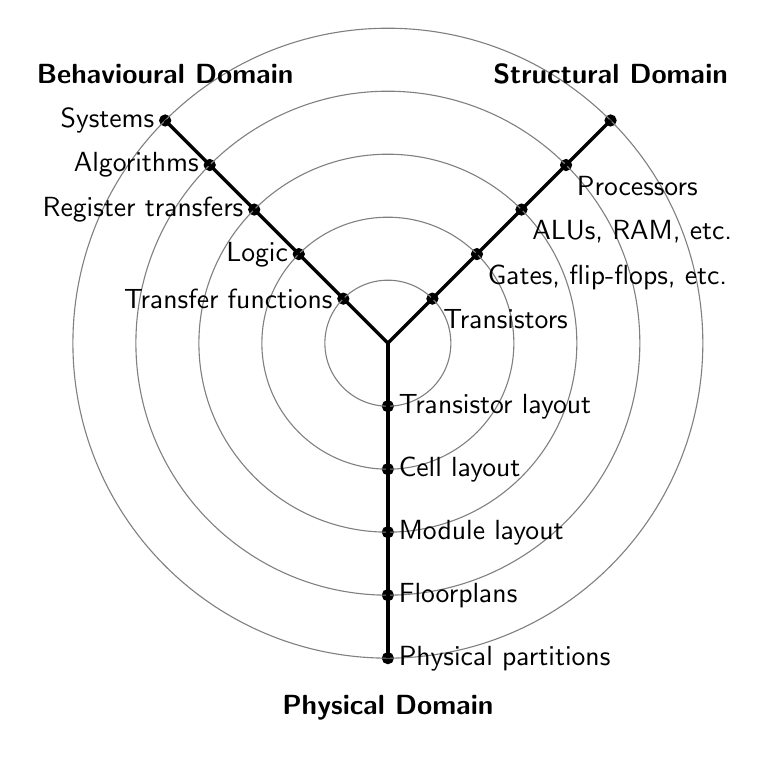
\begin{tikzpicture}[>=stealth',font=\sffamily,auto,on grid]
    %\input{y_chart_common}
    \coordinate (behaviouralNode) at (135:4cm);
    \coordinate (structuralNode) at (45:4cm);
    \coordinate (physicalNode) at (270:4cm);
    \coordinate (originNode) at (0:0cm);

    \draw[fill] (barycentric cs:behaviouralNode=1.0,originNode=0) circle (2pt);
    \draw[fill] (barycentric cs:behaviouralNode=0.8,originNode=0.2) circle (2pt);
    \draw[fill] (barycentric cs:behaviouralNode=0.6,originNode=0.4) circle (2pt);
    \draw[fill] (barycentric cs:behaviouralNode=0.4,originNode=0.6) circle (2pt);
    \draw[fill] (barycentric cs:behaviouralNode=0.2,originNode=0.8) circle (2pt);

    \draw[fill] (barycentric cs:structuralNode=1.0,originNode=0) circle (2pt);
    \draw[fill] (barycentric cs:structuralNode=0.8,originNode=0.2) circle (2pt);
    \draw[fill] (barycentric cs:structuralNode=0.6,originNode=0.4) circle (2pt);
    \draw[fill] (barycentric cs:structuralNode=0.4,originNode=0.6) circle (2pt);
    \draw[fill] (barycentric cs:structuralNode=0.2,originNode=0.8) circle (2pt);

    \draw[fill] (barycentric cs:physicalNode=1.0,originNode=0) circle (2pt);
    \draw[fill] (barycentric cs:physicalNode=0.8,originNode=0.2) circle (2pt);
    \draw[fill] (barycentric cs:physicalNode=0.6,originNode=0.4) circle (2pt);
    \draw[fill] (barycentric cs:physicalNode=0.4,originNode=0.6) circle (2pt);
    \draw[fill] (barycentric cs:physicalNode=0.2,originNode=0.8) circle (2pt);

    \draw[black!50] (0,0) circle (4.0cm);
    \draw[black!50] (0,0) circle (3.2cm);
    \draw[black!50] (0,0) circle (2.4cm);
    \draw[black!50] (0,0) circle (1.6cm);
    \draw[black!50] (0,0) circle (0.8cm);

    \node [above=1em] at (behaviouralNode) {\textbf{Behavioural Domain}};
    \node [above=1em] at (structuralNode) {\textbf{Structural Domain}};
    \node [below=1em] at (physicalNode) {\textbf{Physical Domain}};

    \draw[-, very thick] (behaviouralNode.south) -- (0,0) node[left,pos=0]{Systems} node[left,pos=0.2]{Algorithms} node[left,pos=0.4]{Register transfers} node[left,pos=0.6]{Logic} node[left,pos=0.8]{Transfer functions};

    \draw[-, very thick] (structuralNode.south) -- (0,0) node[pos=0]{ } node[pos=0.2]{Processors} node[pos=0.4]{ALUs, RAM, etc.} node[pos=0.6]{Gates, flip-flops, etc.} node[pos=0.8]{Transistors};

    \draw[-, very thick] (physicalNode.south) -- (0,0) node[right,pos=0]{Physical partitions} node[right,pos=0.2]{Floorplans} node[right,pos=0.4]{Module layout} node[right,pos=0.6]{Cell layout} node[right,pos=0.8]{Transistor layout};

  \end{tikzpicture}
  \caption{Gajski-Kuhn \index{Gajski-Kuhn Y-chart}Y-chart} 
  \label{figure:gajski_kuhn_y_chart__levels_of_abstraction}
\end{figure}

\filbreak

\section{Domain specific languages}

C and C++ are currently the dominant languages for embedded system
programming. It is therefore natural to expect that real-world
embedded cryptography applications be implemented in either of those
two languages. This can lead to hidden and difficult problems to
debug. A lot of cases were left unspecified or undefined in the C or
C++ standard. Hence, compiler implementations have a choice on how to
implement it. The usual approach is to define it as what is most
efficient in terms of the platform. This sacrifices the safety and
portability to ensure efficiency.

\filbreak

\begin{lstlisting}[language=C]
#include <stdio.h>

int b(void) { puts("3"); return 3; }
int c(void) { puts("4"); return 4; }

int main(void)
{
  int a = b() + c();
  printf("%d\n", a);
}
\end{lstlisting}

The evaluation order is unspecified so depending on the compiler, the
output may be 3, 4, 7 or 4, 3, 7. The compiler usually chooses the
optimal way to calculate it given a platform.

The security world does not handle undefined and unspecified values
well. It makes sense to build protections against unsafe, undefined
and unspecified operations into the language. It also makes sense to
make the language easy to learn and understand. This is the common
requirement of a domain specific language, a language tailored for a
specific domain.

%%% Local Variables: 
%%% TeX-PDF-mode: t
%%% TeX-master: "thesis"
%%% End: 


\chapter{Technical preliminaries}

The chapter has the goal of introducing the math and theory behind
formal languages, parsers, algebra, (zero knowledge) proofs of
knowledge.

\section{Formal Languages \cite{Hopcroft}}

\begin{defn}[Alphabet]
  An alphabet $\Sigma$ is a set of symbols.
\end{defn}

\begin{defn}[String]
  A string over an alphabet $\Sigma$ is a sequence of symbols of $\Sigma$.
\end{defn}

\begin{defn}[Concatenation]
  Let $x = a_0 a_1 \dotsm a_n$ and $y = b_0 b_1 \dotsm b_n$, then the
  string $x y = a_0 a_1 \dotsm a_n b_0 b_1 \dotsm b_n$ is the
  concatenation of the strings $x$ and $y$.
\end{defn}

\begin{defn}[Sets]
  The $\Sigma^*$ denotes the set of all the strings over the alphabet
  $\Sigma$, likewise $\Sigma^+$ denotes the set of all the non-empty
  strings over the alphabet $\Sigma$. $$\Sigma^+ \subseteq \Sigma^*
  \setminus \{ \epsilon \}$$ The empty set of strings is denoted
  $\emptyset$.
\end{defn}

\begin{defn}[Language]
  A language over the alphabet $\Sigma$ is a set of strings over
  $\Sigma$. Members of the language are called words of the language.
\end{defn}

\begin{defn}[Concatenation]
  Let $L_1$ and $L_2$ be two languages over alphabet $\Sigma$, the
  language $L_1 L_2 = \{x y | x \in L_1, y \in L_2 \}$ is the
  concatenation of $L_1$ and $L_2$.
\end{defn}

\begin{defn}[Kleene closure]
  Let $L$ be a language over $\Sigma$. Define 
  $$L^0 = \{ \epsilon \}$$
  $$L^i = L L^{i-1} \textrm{for} i \ge 1$$
  the \emph{Kleene closure} of $L$, denoted by $L^*$ is the language:
  $$ L^* = \bigcup_{i \ge 0} L^i $$
  the \emph{positive closure} is
  $$ L^+ = \bigcup_{i \ge 1} L^i $$
  It can be observed that
  $$ L^* = L^+ \cup \{ \epsilon \} $$
  $$ L^+ = L L^* $$
\end{defn}

\subsection{Regular expression}

\begin{defn}[Regular expression]
  A regular expression over $\Sigma$ is defined inductively as follows:
  \begin{enumerate}
  \item $\emptyset$ is a regular expression and represents the empty language
  \item $\epsilon$ is a regular expression and represents the language
    $L = \{ \epsilon \}$
  \item For each $c \in \Sigma$, $c$ is a regular expression and
    represents the language $L = \{ c \}$
  \item For any regular expressions $r$ of language $R$ and $s$ of language $S$:
    \begin{itemize}
    \item $r+s$ is a regular expression representing language $R \cup S$
    \item $r s$ is a regular expression representing language $R S$
    \item $r^*$ is a regular expression representing language $R^*$
    \item $r^+$ is a regular expression representing language $R^+$
    \end{itemize}
  \end{enumerate}
\end{defn}

\begin{thm}
  $r r^*$ can be represented as $r+$
\end{thm}

\begin{proof}
  $r r^*$ represents the language $R R^*$ which is $R^+$
\end{proof}

\subsection{Grammars}

\begin{defn}[Grammar]
  A grammar is a 4-tuple $G = \left< \Sigma, V, S, P \right>$:
  \begin{enumerate}
  \item $\Sigma$ is a finite non-empty set called the \emph{terminal
    alphabet}. The elements of $\Sigma$ are called \emph{terminals}.
  \item $V$ is a finite non-empty set disjoint from $\Sigma$. The
    elements of $V$ are called \emph{non-terminals} or \emph{variables}.
  \item $S \in V$ is a distinguished symbol called the \emph{start symbol}
  \item $P$ is a finite set of \emph{productions (rules)} of the form
    $$ \alpha \rightarrow \beta $$
    $$ \alpha \in (\Sigma \cup V)^* V (\Sigma \cup V)^* $$
    $$ \beta \in (\Sigma \cup V)^* $$
  \end{enumerate}
\end{defn}

\begin{defn}[Context-free grammar]
  The grammar $G$ is a context free grammar if $|\alpha|$ = 1 ($\alpha = V$).
\end{defn}

\begin{defn}[LL grammar]
  A context free grammar $G$ is an LL grammar if $\beta \in \Sigma
  (\Sigma \cup V)^*$
\end{defn}

\section{Montgomery Product}

Modular multiplications would involve trial division after the
multiplication step were it not for the algorithm know as Montgomery
product invented by Peter L. Montgomery \cite{Montgomery}.

The basic step and the property of the algorithm is computing the
residues modulo $N$.

\begin{defn}
  Define an radix $R$ such that $R R^{-1} - N N' = 1$. The residue
  $\overline{a}$ of $a$ is $\overline{a} = a R$
\end{defn}

\begin{thm}
  The algorithm for Montgomery reduction is
  \begin{algorithm}[hbt!]
    \caption{Montgomery reduction}
    \begin{algorithmic}
      \Function{Reduce}{$T$}
      \State $m \gets (T \bmod{R}) N' \bmod{R}$
      \State $t \gets (T + m N)/R$
      \If{$t \ge N$} \Return $t - N$
      \Else \, \Return $t$
      \EndIf
      \EndFunction
    \end{algorithmic}
  \end{algorithm}
\end{thm}
\begin{proof}
  Assume $T < R$, then
  \begin{align*}
      m & = T N' \\
    m N & = T N' N \\
        & = T R R^{-1} - T \\
        & = - T \bmod{R} \\
    t R & = T + m N \\
        & = T \bmod{N}
  \end{align*}
\end{proof}

To compute the Montgomery product, one can now apply the reduction to
the product of the reduced $\overline{a}$ and $\overline{b}$:
\begin{algorithmic}
  \Function{MontgomeryProduct}{$\overline{a}$, $\overline{b}$}
    \State $t \gets \overline{a} \cdot \overline{b}$
    \State \Return \Call{Reduce}{$t$}
  \EndFunction
\end{algorithmic}

Ko\c{c} goes a step further and inlines the reduction to see possible
optimizations when implementing the algorithm on multiple
architectures \cite{Koc}:

\begin{algorithm}[hbt!]
  \begin{algorithmic}
    \Function{MontgomeryProduct}{$\overline{a}$, $\overline{b}$}
      \State $m \gets (\overline{a} \cdot \overline{b} \bmod{R}) N' \bmod{R}$
      \State $t \gets (\overline{a} \cdot \overline{b} + m N)/R$
      \If{$t \ge N$} \Return $t - N$
      \Else \, \Return $t$
      \EndIf 
   \EndFunction
  \end{algorithmic}
\end{algorithm}

If such a primitive is provided on an architecture, the reduction then
becomes:

\begin{algorithm}
  \begin{algorithmic}
    \Function{MontgomeryReduce}{$T$}
      \State \Return \Call{MontgomeryProduct}{$T$, $R^2$}
    \EndFunction
  \end{algorithmic}
\end{algorithm}

Montgomery product eliminates the trial division. It does so at the
expense of computing the residues. However, these residues can be
precomputed in the beginning. Then, for a sufficient number of
Montgomery multiplications, the amortized cost is negligible. The
problem of computing the modular product is then given by:
\begin{enumerate}
\item Transform into the Montgomery domain
\item Compute the product in the Montgomery domain
\item Transform the result back into the integer domain
\end{enumerate}
This is also depicted in Figure \ref{fig:montpro_flow} where both paths
are shown when starting from the integer domain.

\begin{figure}[hbt!]
  \centering
  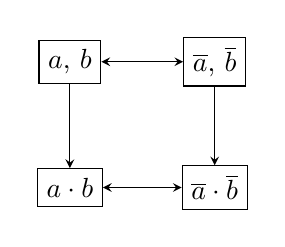
\begin{tikzpicture}[>=stealth]
    \tikzstyle{dom}=[rectangle,draw=black,thin,align=center]

    \node[matrix, column sep=1cm, row sep=1cm](matrix){
      \node[dom](intd){$a$, $b$}; & \node[dom](montd){$\overline{a}$, $\overline{b}$}; \\
      \node[dom](intpro){$a \cdot b$}; &\node[dom](montpro){$\overline{a} \cdot \overline{b}$}; \\
    };

    \draw[<->] (intd) -- (montd);
    \draw[->] (montd) -- (montpro);
    \draw[<->] (montpro) -- (intpro);
    \draw[->] (intd) -- (intpro);
  \end{tikzpicture}
  \caption{Montgomery product flow}
  \label{fig:montpro_flow}
\end{figure}

\filbreak

\section{Turing Machine}

A Turing machine is a mathematical model of computation \cite{Turing}.
Informally, it consists of:
\begin{itemize}
\item A tape divided into cells
\item A head that reads and writes
\item A finite table (action table or transition function)
\item A state
\end{itemize}

\begin{figure}[hbt!]
\centering
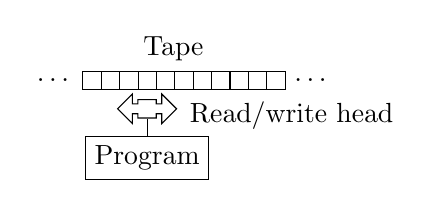
\begin{tikzpicture}[
      start chain=1 going right,start chain=2 going below,node distance=-0.15mm
    ]
    \node [on chain=2] {Tape};
    \node [on chain=1] at (-1.5,-.4) {\ldots};  
    \foreach \x in {1,2,...,11} {
        \x, \node [draw,on chain=1] {};
    } 
    \node [name=r,on chain=1] {\ldots}; 
    \node [name=k, arrow box, draw,on chain=2,
        arrow box arrows={east:.25cm, west:0.25cm}] at (-0.335,-.65) {};    
    \node at (1.5,-.85) {Read/write head};
    \node [on chain=2] {};
    \node [draw,on chain=2] {Program};
    \chainin (k) [join];
\end{tikzpicture}
\caption{Turing machine}
\label{fig:turing}
\end{figure}

A more formal definition comes from Hopcroft \cite{Hopcroft}. A Turing machine
is defined as a 7-tuple $M = \left< Q, \Gamma, b, \Sigma, q_0, F, \delta \right>$
\begin{itemize}
\item $Q$ is a finite, non-empty set of states
\item $\Gamma$ is a finite, non-empty set of the tape alphabet/symbols
\item $b \in \Gamma$ is the blank smybol
\item $\Sigma \subseteq \Gamma \setminus \{ b \}$ the set of input symbols
\item $q_0 \in Q$ is the initial state
\item $F \subseteq Q$ is the set of final or accepting states
\item $\delta : Q \setminus F \times \Gamma \rightarrow Q \times \Gamma \times \{ L,R \}$ is the transition relation
\end{itemize}

\section{Zero Knowledge Proofs of Knowledge}

Sometimes one party wants to prove knowing a secret to the other party
but without actually revealing that secret. Let's take a corporate
espionage example. Suppose that we wish to buy a secret but are not
convinced of the seller's honesty (he may leave us without money and
run away with our secret). We then devise a protocol by which we can
be convinced that the seller knows the secret.

\filbreak

To define a proof a knowledge it is convenient to use a Turing
machine. In this case let's define an interactive Turing machine (ITM)
with 5 tapes:
\begin{itemize}
\item Input tape (read-only)
\item Receiving tape (read-only)
\item Sending tape (write-only)
\item Output tape (write-only)
\item Working tape (read-write)
\end{itemize}

An interactive protocol is an ordered pair of ITMs that share the same
input tape, and have receiving and sending tapes cross-connected
(sending to receiving, receiving to sending).

An interactive proof system can be represented by the following two
properties:
\begin{itemize}
\item Completeness $(x,w) \in \mathcal{R} \Rightarrow P(accept) > \frac{2}{3}$
\item Soundness $(x,w) \notin \mathcal{R} \Rightarrow P(accept) < \frac{1}{3}$
\end{itemize}

Informally, the previous two properties state that
\begin{itemize}
\item if a statement is true, a honest prover will be able to convince the verifier of the validity with a large probability
\item if a statement is false, no dishonest prover will be able to convince the verifier of the validity with a probability larger than the threshold
\end{itemize}

To make it a zero-knowledge an additional property is needed. We can
state that the prover should not release any knowledge on the secret
it possesses. To make it more formal, we state that a third party
should not be able to distinguish between a successful communication
and an unsuccessful one. Depending on how indistinguishable it is, we
can differentiate three cases:
\begin{itemize}
\item perfectly indistinguishable
\item statistically indistinguishable
\item computationally indistinguishable
\end{itemize}

\section{Data Flow Graph and Control Flow Graph}

An algorithm is completely and uniquely defined by its Data Flow Graph (DFG),
whereas the implementation of an algorithm is what gives it its Control Flow
Graph (CFG).

The usual step in converting an algorithm in software to an algorithm
in hardware is to extract the DFG \cite{Schaumont}.

%%% Local Variables: 
%%% TeX-PDF-mode: t
%%% TeX-master: "thesis"
%%% End: 


\chapter{Existing Frameworks and Tools}

The goal of this chapter is to review existing frameworks for
implementing Zero Knowledge Proofs of Knowledge as well as tools that
will be used to design our custom framework.

The chapter starts by analyzing CACE Project Zero Knowledge Compiler,
which will be the basis of our custom framework. A brief overview of
the framework is given followed by the Protocol Specification Language
(PSL) and the Protocol Implementation Language (PIL) overview. More
attention is given to PIL since it will be the language of choice of
our custom framework.

A brief description of related frameworks follows, namely ZKPDL and
ZKCrypt. Only a short overview is given and a high-level comparison
with our custom framework. The chapter then continues on describing
tools that will be used to build our custom framework:
\begin{itemize}
\item ANTLR is a parser generator tool producing LL(*) parsers, we
  will use it to construct a PIL parser which will be the front-end of
  our framework.
\item LLVM is a compiler infrastructure framework that has recently
  seen wide use in many fields relating to computer science. We will
  use it as a middle layer along with its intermediate language LLVM
  IR.
\item GMP is a popular multi-precision library used within the CACE
  ZKC. The changes that will be introduced to PIL later on will make
  it incompatible with the CACE ZKC, therefore we need to provide this
  implementation as well.
\item GEZEL is a cycle-true cosimulation environment and a hardware
  description language. We will target GEZEL language in our
  framework, allowing us to perform HW-SW co-design.
\end{itemize}

\section{CACE Project Zero Knowledge Compiler}
\label{sec:cace}

\subsection{Framework Overview}

The CACE (Computer Aided Cryptography Engineering)
Project\footnote{http://www.cace-project.eu} was an European project
aiming at developing a toolbox for security software. It attempted to
ease the creation of cryptographic software for those outside the
domain by setting the following goals:
\begin{itemize}
\item Automatic translation from natural specification - the
  term natural is taken from the user's perspective, meaning something
  ``natural'' for the user, not dwelling too much into the specific
  niches of cryptography, giving an abstract overview
\item Automatic security awareness, analysis and corrections - to be
  able to detect side channels that are unintentionally introduced,
  warn the user and offer corrective actions
\item Automatic optimization for diverse platforms - different
  platforms are suited for different operations, assume different
  usage patterns etc\ldots, the toolbox should be as most insensitive
  as it can to the platform it is implemented on
\end{itemize}

Apart from these goals that deal with the end-user, the project had
strategic goals of opening a new field of research and promoting
automatic tools when it came to cryptography software. The project
itself was split into multiple working groups:
\begin{itemize}
\item WP1 Automating Cryptographic Implementation - dealing with the
  low level crypto operations, searching and identifying side channel
  attacks, providing a domain specific language
\item WP2 Accelerating Secure Network - dealing with basic operations
  for module intercommunication
\item WP3 Bringing Proofs of Knowledge to Practice - dealing with
  implementing a compiler for Proofs of Knowledge
\item WP4 Securing Distributed Management of Information - dealing
  with higher operations for module intercommunication
\item WP5 Formal Verification and Validation - dealing with analysis
  of the correctness, assuring the user of the protocol validity
\end{itemize}

The WP3 working group is of the importance for this thesis as it deals
directly with proofs of knowledge. The end result of the working group
was a compiler along with a specification language (PSL) and an
intermediate language (PIL). Figure \ref{fig:cace_workflow} depicts the
typical flow of the CACE ZKPK Compiler:
\begin{enumerate}
\item The ZKPK to be implemented is specified in Protocol
  Specification Language (PSL). PSL is based on Camenisch-Stadler
  notation (see Sub-subsection \ref{subsubsec:camenisch_stadler}) and
  allows the specification of complex $\Sigma$ protocols in an easy way.

\item The Protocol Compiler transforms the specification in PSL into
  an implementation in Protocol Implementation Language (PIL). PIL is
  a Turing-complete language on its own and it also allows for
  automated verification.

\item The framework transforms PIL code into an implementation in C or
  Java that can be compiled and executed on a target architecture. Two
  modules are generated along with an additional support library
  providing math and communication. The two modules are a prover and a
  verifier, using network sockets for communication.

\item The PIL code is verified using the Protocol Verification Toolbox
  (PVT). On input the specification in PSL and the implementation in
  PIL, PVT employs the theorem prover Isabelle/HOL \cite{isabelle_hol}
  to create a proof of the soundness guarantees of the generated ZKPK
  implementation.

\item  Human readable documentation in \LaTeX{} is also generated from PIL code.

\end{enumerate}

\begin{figure}[hb!]
  \centering
  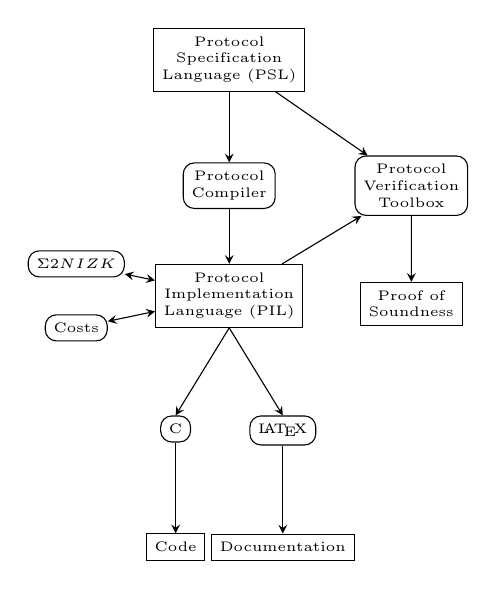
\begin{tikzpicture}[>=stealth,level distance=1.5cm,font=\tiny]
    \tikzstyle{edge from parent}=[draw,->]

    \Tree [.\node[language](psl){Protocol \\ Specification \\ Language (PSL)};
      [.\node[compiler](pc){Protocol \\ Compiler};
        [.\node[language](pil){Protocol \\ Implementation \\ Language (PIL)};
          [.\node[compiler](c){C}; \node[language](code){Code};]
          [.\node[compiler](latex){\LaTeX}; \node[language](doc){Documentation};]
        ]
      ]
    ]

    \node[compiler] (pvt)         [right=of pc,anchor=west]          {Protocol \\ Verification \\ Toolbox}
    child {node[language] {Proof of \\ Soundness}};

    \node[compiler] (sigma) [left=of pil.north west,anchor=center] {$\Sigma 2 N I Z K$};
    \node[compiler] (cost) [left=of pil.south west,anchor=center] {Costs};

    \draw[<->] (sigma) -- (pil);
    \draw[<->] (cost) -- (pil);

    \draw[->] (psl) -- (pvt);
    \draw[->] (pil) -- (pvt);
  \end{tikzpicture}
  \caption{CACE Project Zero Knowledge Compiler typical workflow \cite{CACE}}
  \label{fig:cace_workflow}
\end{figure}

\subsection{PSL}
\label{subsec:psl}

The Protocol Specification Language (PSL) is a high level language of
CACE Project WP3 for specifying Proofs of Knowledge based on
Camenisch-Stadler notation, allowing specification of complex $\Sigma$
protocols \cite{CACE, yaczk}. PSL is best explained following an
example of a simple protocol, Schnorr's Identification Protocol (see
Sub-subsection \ref{subsubsec:schnorr_protocol}). We start from the
Camenisch-Stadler notation for Schnorr's Identification Protocol:
\[
  \textrm{ZPK}\left[ (x): y = g^x \right]
\]
The PSL language is structured into blocks, and for the Schnorr
example the blocks are as follows:
\begin{itemize}
\item Declarations - specifying all the variables used within
  the protocol
\begin{lstlisting}[language=PSL]
Declarations {
  Prime(1024) p;
  Prime(160) q;
  Zmod+(q) x;
  Zmod*(p) g, y;
}
\end{lstlisting}
  This example shows how to declare prime numbers as well as elements
  of a residue group. Here, $p$ is declared as a prime of $1024$ bits
  and $q$ is declared as a prime of $160$ bits, $x \in Z_q^+$ and $g,
  y \in Z_p^*$.
\item Input - specifying which of the variables are public and which
  are private (to the Verifier or the Prover)
\begin{lstlisting}[language=PSL]
Inputs {
  Public := y,p,q,g;
  ProverPrivate := x;
}
\end{lstlisting}
  This example shows how to specify which are public known variables
  and which are known only to the prover. It is also possible to
  specify a variable known only to the verifier.
\item Properties - specifying the properties of the protocol
\begin{lstlisting}[language=PSL]
Properties {
  KnowledgeError := 80;
  SZKParameter := 80;
  ProtocolComposition := P_1;
}
\end{lstlisting}
  This example shows how to specify the knowledge error, which is
  $2^{-80}$ in this case. The tightness is specified at $2^{-80}$ as
  well. The protocol composition allows to specify multiple protocols
  via AND, OR and XOR. Since this is a simple case, only one protocol is
  used.

\item Specifying the protocols itself (the homomorphism to
  use and the relation to be proven)
\begin{lstlisting}[language=PSL]
SigmaPhi P_1 {
  Homomorphism (phi : Zmod+(q) -> Zmod*(p) : (a) |-> (g^a));
  ChallengeLength := 80;
  Relation ((y) = phi(x));
}
\end{lstlisting}
  The relation to be proven is $y = g^x$ which is specified as the
  homomorphism $\phi(a) : Z_q^+ \rightarrow Z_p^* := g^a$. The
  ChallengeLength allows to customize the protocol for certain
  devices.  The generated protocol will be repeated until the required
  knowledge error is met. For example, a challenge length of $1$ will
  repeat the protocol $80$ times to satisfy the knowledge error of
  $2^{-80}$.

\end{itemize}

The previous blocks combined give a complete PSL specification of
Schnorr's Identification Protocol:
\lstinputlisting[language=PSL]{example.psl}

\subsection{PIL}
\label{subsec:pil}

The Protocol Implementation Language (PIL) is the low
level/intermediate language of CACE ZKPK Compiler. The language itself
gives all the rounds and computations of a protocol and is meant to be
easy to understand and learn, aiding verification of correctness from
a user's point of view. PIL is also Turing-complete with completely
specified semantics allowing automatic verification. The following
features are supported in PIL:
\begin{itemize}
\item global shared constants (parameters)
\begin{lstlisting}[language=PIL]
Common (
Z l_e = 1024;
Z SZKParameter = 80;
Prime(1024) n
) {
...
}
\end{lstlisting}

\item global constants (parameters)
\begin{lstlisting}[language=PIL]
Prover (
Zmod+(q) x;
Zmod+(q) v
) {
...
}
\end{lstlisting}

\item global variables
\begin{lstlisting}[language=PIL]
Prover (
...
) {
Zmod+(q) s, r;
...
}
\end{lstlisting}

\item conditionals
\begin{lstlisting}[language=PIL]
IfKnown(...) {

} Else {

}
\end{lstlisting}

\item loops
\begin{lstlisting}[language=PIL]
For i In [1,2] {
  ...
}
\end{lstlisting}

\item functions
\begin{lstlisting}[language=PIL]
Def (Zmod*(p) _t_1): Round1(Void) {
 _r_1 := Random(Zmod+(q));
 _t_1 := (g^_r_1);
}
\end{lstlisting}

\item predicates
\begin{lstlisting}
x := Random(Zmod+(q));
CheckMembership(x, Zmod+(q));
Verify(x == x);
\end{lstlisting}

\item type alias
\begin{lstlisting}
_C = Int(80) _c;
\end{lstlisting}

\end{itemize}

Proof entities are specified as blocks and there is always a Common
block with declarations and definitions visible to all other
blocks. Each block can define multiple functions, each having inputs
and outputs and consisting of assignments, loops or conditional
flow. The execution order is specified via block function pairs:
\begin{lstlisting}[language=PIL]
ExecutionOrder := (Prover.Round0, Verifier.Round0, Prover.Round1, Verifier.Round1, Prover.Round2, Verifier.Round2);
\end{lstlisting}
The communication itself is specified via these functions with inputs
of the current function matching the output of the previous
function. For example, the outputs of Round0 from Prover match the
inputs of Round0 from Verifier.

Again, the Schnorr protocol is used as an example, automatically
generated from the PSL that was given in Sub-section \ref{subsec:psl}.
\lstinputlisting[language=PIL]{example.pil}

\section{Related Frameworks}

Although the CACE Project Zero Knowledge Compiler (CACE ZKC) will be
the framework of choice for extension in this thesis, ZKPDL and
ZKCrypt will be presented as well for the sake of completeness. It is
mostly a brief overview along with a brief comparison with CACE ZKC.

\subsection{ZKPDL/Cashlib}

ZKPDL is a ZKPK description language used by the Cashlib framework to
implement e-cash. The framework uses an interpreter based approach and
applies result caching to speed up computations. Unlike PIL, ZKDPL is
not Turing-complete and only supports non-interactive proofs of
knowledge \cite{zkpdl}. ZKPDL does allow generation of parameters
which PIL lacks \cite{yaczk} but this can be mitigated by defining and
using constant expressions.

\subsection{ZKCrypt}
\label{subsec:zkcrypt}

ZKCrypt is a framework built atop the CACE ZKC framework
\cite{zkcrypt}. It leverages
CertiCrypt\footnote{http://www.msr-inria.inria.fr/projects/sec/certicrypt/index.html}
to produce a formal assurance of the correctness. Where CACE only
allows proof of soundness using Isabelle/HOL, ZKCrypt allows formal
assurance of the implementation satisfying completeness, proof of
knowledge and zero knowledge properties.

ZKCrypt generates formal evidence of each of the CACE ZKC compilation
steps except code generation and, as such, is complementary to the
framework developed within the course of this thesis.

\section{Other Tools}

\subsection{ANTLR}

ANTLR\footnote{http://www.antlr.org} (ANother Tool For Language
Recognition) is a parser generator tool that generates LL(*)
parsers. The tool accepts grammar definitions as input files and
produces output in the target language which can be chosen among C,
Java or Python.

The input to ANTLR is a context-free grammar that must be of the LL
form. This means that there should be no left recursion or ambiguities
when encountering the first element on the left. Left factoring is
usually used to solve this, but this can sometimes lead to rules which
have counter intuitive representation. The grammar can be augmented with
syntactic and semantic predicates to cope with this \cite{ANTLR,ANTLR2}.

ANTLR can generate both lexers and parser. The two grammars can be
combined in a single file.  In such cases, parser rules are written in
lowercase, while the lexer rules are written in uppercase. Upon
generation, two separate entities will be created, a parser source and
a lexer source in the target language (as illustrated in Figure
\ref{fig:antlr_parser_lexer}).

\begin{figure}[hb!]
  \centering
  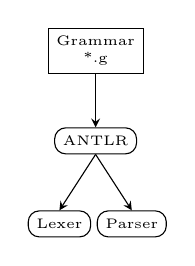
\begin{tikzpicture}[>=stealth, font=\tiny]
    \tikzstyle{edge from parent}=[draw,->]

    \Tree[.\node[language](parser_g){Grammar \\ *.g};
      [.\node[compiler](antlr){ANTLR};
        [.\node[compiler](lexer){Lexer};]
        [.\node[compiler](parser){Parser};]
      ]
    ]
  \end{tikzpicture}
  \caption{ANTLR Parser/Lexer generation}
  \label{fig:antlr_parser_lexer}
\end{figure}

The output of the parser generated by ANTLR is a Parse Tree. ANTLR
also allows specifying a tree transformation to apply to this Parse
Tree. This can be used to automatically generate an Abstract Syntax
Tree (AST).

ANTLR can also generate a tree parser/walker that visit each node of
the AST and applies a certain operation or produces a certain
output. The generation of such a walker is illustrated in Figure
\ref{fig:antlr_tree_walker}.

\begin{figure}[hb!]
  \centering
  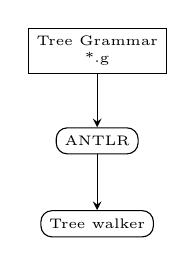
\begin{tikzpicture}[>=stealth, font=\tiny]
    \tikzstyle{edge from parent}=[draw,->]

    \Tree[.\node[language](parser_g){Tree Grammar \\ *.g};
      [.\node[compiler](antlr){ANTLR};
        [.\node[compiler](lexer){Tree walker};]
      ]
    ]
  \end{tikzpicture}
  \caption{ANTLR Tree walker generation}
  \label{fig:antlr_tree_walker}
\end{figure}

\subsection{LLVM}
\label{subsec:llvm}

LLVM\footnote{http://llvm.org} is a compiler framework designed to
support transparent, life-long program analysis and transformation for
arbitrary programs, by providing high-level information to compiler
transformations at compile-time, link-time, run-time, and in idle time
between runs \cite{LLVM:CGO04}.

Traditional compilers were tailored for only a few languages (with the
exception of GCC). However, all traditional compilers suffer from the
large inter-dependency of the basic blocks (Front-end, Optimizer,
Back-end). LLVM tries to solve this by providing an intermediate form
called the LLVM IR. A typical flow involving the basic blocks is
depicted in Figure \ref{fig:llvm_flow}.

\begin{figure}[hb!]
  \centering
   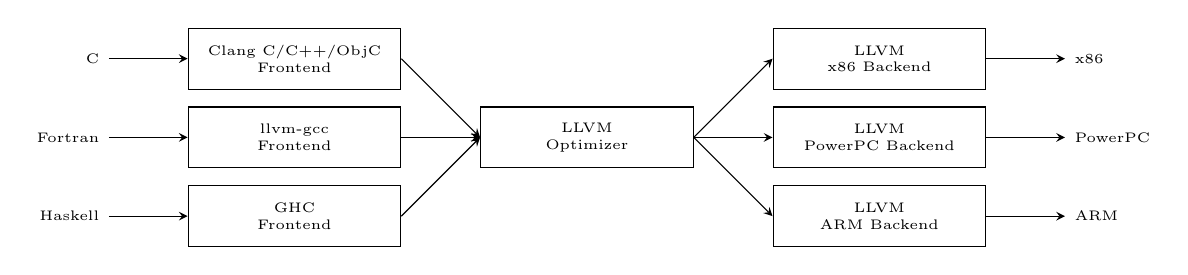
\begin{tikzpicture}[>=stealth]
    \tikzstyle{lang}=[rectangle,draw=black,thin,font=\tiny,inner
    sep=0pt, align=center,minimum width=2.7cm,minimum height=2.2em]

    \tikzstyle{txt}=[font=\tiny]

    \node[lang](llvm_opt){LLVM \\ Optimizer};
    \node[lang](ppc_back)[right=1 cm of llvm_opt]{LLVM \\ PowerPC Backend};
    \node[txt](ppc)[right=of ppc_back]{PowerPC};
    \node[lang](x86_back)[above of=ppc_back]{LLVM \\ x86 Backend};
    \node[txt](x86)[right=of x86_back]{x86};
    \node[lang](arm_back)[below of=ppc_back]{LLVM \\ ARM Backend};
    \node[txt](arm)[right=of arm_back]{ARM};

    \node[lang](gcc_front)[left=1 cm of llvm_opt]{llvm-gcc \\ Frontend};
    \node[txt](fortran)[left=of gcc_front]{Fortran};
    \node[lang](clang_front)[above of=gcc_front]{Clang C/C++/ObjC \\ Frontend};
    \node[txt](c)[left=of clang_front]{C};
    \node[lang](ghc_front)[below of=gcc_front]{GHC \\ Frontend};
    \node[txt](haskell)[left=of ghc_front]{Haskell};

    \draw[->] (clang_front.east) -- (llvm_opt.west);
    \draw[->] (gcc_front.east) -- (llvm_opt.west);
    \draw[->] (ghc_front.east) -- (llvm_opt.west);

    \draw[->] (llvm_opt.east) -- (x86_back.west);
    \draw[->] (llvm_opt.east) -- (ppc_back.west);
    \draw[->] (llvm_opt.east) -- (arm_back.west);

    \draw[->] (x86_back) -- (x86);
    \draw[->] (ppc_back) -- (ppc);
    \draw[->] (arm_back) -- (arm);

    \draw[->] (c) -- (clang_front);
    \draw[->] (fortran) -- (gcc_front);
    \draw[->] (haskell) -- (ghc_front);
  \end{tikzpicture}
  \caption{LLVM typical workflow \cite{llvm_general}}
  \label{fig:llvm_flow}
\end{figure}

Due to its modularity, LLVM has recently seen increased usage in a number
of independent fields:
\begin{itemize}
\item implementing a C/C++ compiler (Clang)
\item implementing C-to-HDL translation
\item implementing a Haskell compiler (GHC)
\item implementing Secure Virtual Architectures (SVA)
\item implementing dynamic translation
\item implementing OpenGL drivers (Mac OS X)
\item implementing OpenCL drivers (AMD)
\end{itemize}

\subsubsection{LLVM IR}

The LLVM IR is the intermediate representation language of the LLVM
project. On its own it is a first-class language with well defined
semantics \cite{llvm_general, llvm_master_thesis}. Variables are in
the SSA (Static Single Assignment) form meaning that they can be only
assigned once and they keep that value for their entire lifetime. All
the values residing in memory need to be loaded to a variable first
and stored back to memory if they wish to be saved. Instructions
operate solely upon variables. In this respect, the LLVM IR resembles
the assembly language of an infinitely many registers Load-Store based
RISC processor. The following snippet, taken from \cite{llvm_general},
demonstrates how two different functions implemented in C (one without
recursion and one with recursion) are compiled to LLVM IR:

\begin{lstlisting}[language=C]
unsigned add1(unsigned a, unsigned b) {
  return a+b;
}

unsigned add2(unsigned a, unsigned b) {
  if (a == 0) return b;
  return add2(a-1, b+1);
}
\end{lstlisting}

\begin{lstlisting}
define i32 @add1(i32 %a, i32 %b) {
entry:
  %tmp1 = add i32 %a, %b
  ret i32 %tmp1
}

define i32 @add2(i32 %a, i32 %b) {
entry:
  %tmp1 = icmp eq i32 %a, 0
  br i1 %tmp1, label %done, label %recurse

recurse:
  %tmp2 = sub i32 %a, 1
  %tmp3 = add i32 %b, 1
  %tmp4 = call i32 @add2(i32 %tmp2, i32 %tmp3)
  ret i32 %tmp4

done:
  ret i32 %b
}
\end{lstlisting}

A central concept while constructing LLVM IR is the
\emph{Module}~\cite{llvm_ir}, corresponding loosely to a source
file. A \emph{Module} consists of functions, global variables and
symbol table entries.

\subsection{GMP}
\label{subsec:gmp}

GMP\footnote{http://gmplib.org/} is a multi-precision library
supporting signed integers, rational numbers and floating-point
numbers with precision limited only the available memory. The library
provides a consistent calling interface across the different
supporting types. Main target applications of the library are
cryptography and computer algebra systems. The library itself aims to
be highly efficient by using different algorithms for different
operand sizes as well as extensive use of inline assembly and
additional processor instruction sets.

\subsection{GEZEL}
\label{subsec:gezel}

GEZEL is a cycle-accurate hardware description language (HDL) using the
Finite-State-Machine + Datapath (FSMD) model \cite{gezel}.

The basic element is a Signal Flow Graph. It groups operations that
are to be executed concurrently in the same clock cycle.
\begin{lstlisting}[language=GEZEL]
sfg increment {
  a = a + 1;
}
\end{lstlisting}
One or more of these SFGs are used to form a datapath which is the
main building block. It is the smallest GEZEL unit that can stand on
its own and be simulated \cite{gezel}. A datapath can be thought of as
a \emph{module} in Verilog or an \emph{entity} in VHDL. Here is a
full contained example of a counter in GEZEL:
\begin{lstlisting}[language=GEZEL]
dp counter(out value : ns(2)) {
   reg c : ns(2);
   always {
     value = c;
     c = c + 1;
     $display("Cycle ", $cycle, ": counter = ", value);
   }
}

system S {
  counter;
}
\end{lstlisting}

Figure \ref{fig:gezel_workflow} shows how the GEZEL language
can be used as an input to:
\begin{itemize}
\item fdlvhd - a generator that can generate synthesizeable VHDL or
  Verilog
\item fdlsim - a cycle accurate simulator used to verify and validate
  the design
\item gplatform - a co-simulation tool used for HW/SW co-design purposes
\end{itemize}

\begin{figure}[hb!]
  \centering
  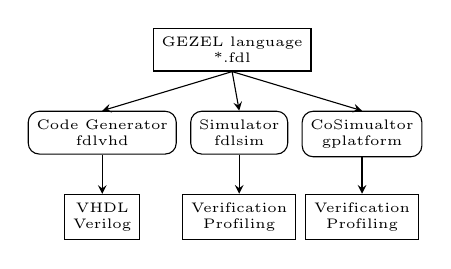
\begin{tikzpicture}[>=stealth, font=\tiny]
    \tikzstyle{edge from parent}=[draw,->]

    \Tree[.\node[language](fdl){GEZEL language \\ *.fdl};
      [.\node[compiler](fdlvhd){Code Generator \\ fdlvhd};
        [.\node[language](vhdl){VHDL \\ Verilog};]
      ]
      [.\node[compiler](fdlsim){Simulator \\ fdlsim};
        [.\node[language](sim){Verification \\ Profiling};]
      ]
      [.\node[compiler](gplatform){CoSimualtor \\ gplatform};
        [.\node[language](cosim){Verification \\ Profiling};]
      ]
    ]
  \end{tikzpicture}
  \caption{GEZEL workflow \cite{gezel}}
  \label{fig:gezel_workflow}
\end{figure}

The co-simulation tool allows to cosimulate GEZEL designs with
instruction-set simulations \cite{gezel}. Supported processors are
ARM, AVR, 8051, MicroBlaze and PicoBlaze. The cosimulation tool allows
for designing a processor-coprocessor pair for a general purpose
processor and a custom dedicated coprocessor.

%%% Local Variables:
%%% TeX-PDF-mode: t
%%% TeX-master: "thesis"
%%% End:


\chapter{Custom Framework}

This chapter aims to present the custom framework that was developed
within the course of this thesis. It starts with the motivation of
domain specific languages then gives the reasoning to extend the CACE
Project Zero Knowledge Compiler. Figure
\ref{fig:custom_framework_workflow} gives an overview of the custom
extensions. They are presented in detail in Section
\ref{sec:cace_extensions}. All of targets except for GEZEL come from
LLVM so the GEZEL target will also be covered.

\begin{figure}[hb!]
  \centering
  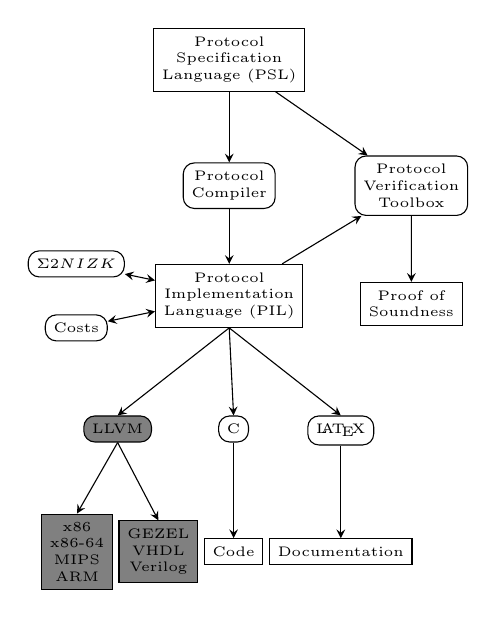
\begin{tikzpicture}[>=stealth,level distance=1.5cm, font=\tiny]
    \tikzstyle{edge from parent}=[draw,->] \tikzset{every leaf
      node/.style={anchor=center}}

    \Tree [.\node[language](psl){Protocol \\ Specification \\ Language (PSL)};
      [.\node[compiler](pc){Protocol \\ Compiler};
        [.\node[language](pil){Protocol \\ Implementation \\ Language (PIL)};
          [.\node[compiler,added](llvm){LLVM};
            \node[language,added](asm){x86 \\ x86-64 \\ MIPS \\ARM};
            \node[language,added](gezel){GEZEL \\ VHDL \\ Verilog};
          ]
          [.\node[compiler](c){C}; \node[language](code){Code};]
          [.\node[compiler](latex){\LaTeX}; \node[language](doc){Documentation};]
        ]
      ]
    ]

    \node[compiler] (pvt)         [right=of pc,anchor=west]          {Protocol \\ Verification \\ Toolbox}
    child {node[language] {Proof of \\ Soundness}};

    \node[compiler] (sigma) [left=of pil.north west,anchor=center] {$\Sigma 2 N I Z K$};
    \node[compiler] (cost) [left=of pil.south west,anchor=center] {Costs};

    \draw[<->] (sigma) -- (pil);
    \draw[<->] (cost) -- (pil);

    \draw[->] (psl) -- (pvt);
    \draw[->] (pil) -- (pvt);
  \end{tikzpicture}
  \caption{Custom framework (extensions to CACE Zero Knowledge
    Compiler highlighted)}
  \label{fig:custom_framework_workflow}
\end{figure}

\section{Motivation}

\subsection{Domain Specific Language}

C is not a very safe language for cryptography applications. This
can be seen already from the goal of C which was to design a
``portable'' assembler. The design choice was not to sacrifice
efficiency so some things are intentionally left undefined or
unspecified in the standard. It is left to the end compilers to
implement it as they choose. The usual choice is just to implement in
the most efficient way for the target platform. For example, the
following code uses this unspecified behavior:

\begin{lstlisting}[language=C]
#include <stdio.h>

int b(void) { puts("3"); return 3; }
int c(void) { puts("4"); return 4; }

int main(void)
{
  int a = b() + c();
  printf("%d\n", a);

  return 0;
}
\end{lstlisting}

The evaluation order is unspecified so depending on the compiler and
the platform, the output may be 3, 4, 7 or 4, 3, 7. The crypto world
should not have undefined nor unspecified behaviors so this is why a
domain specific language is a key point of this thesis.

A domain specific languages hides all the operations that are deemed
not important and allows an abstract overview of the operations. This

\subsection{Extending CACE Zero Knowledge Compiler}

The C code generated by CACE uses GNU GMP, which is a multi-precision
arithmetic library. This library is tailored for desktop computers and
is not well suited for small embedded devices. Separation of the
supporting library allows plugging in of a custom multi-precision
library but this is impractical. There are various devices available
and writing a multi-precision library for each of them is error prone
and inefficient. 

The fact that the CACE Project Zero Knowledge Compiler already uses
its own domain specific language makes it a useful candidate for
extension. It is possible to use LLVM as a low level language and
assure portability and type strictness.

ZKPDL also has its own domain specific language. However, the approach
of creating an interpreter is considered too inefficient for embedded
devices.

As the CACE project is deemed more suited for the task, the custom
framework will extend CACE. LLVM already allows for
\begin{itemize}
\item Interpreted code - by using its interpreter
\item JIT (Just In Time) compiled code - by compiling the code at runtime
\item Compiled code - by allowing to code to be compiled later on
\end{itemize}
Also, since the intermediate form of LLVM is of the SSA (Static Single
Assignment) form, it is believed that more aggressive optimizations
are possible. Since the DFG (Data Flow Graph) can be easily extracted
from the SSA form, hardware realizations are also made possible.

\section{Extensions to GEZEL}

\subsection{Terminal communication ipblocks}

A modification to GEZEL was needed to allow interactivity. A terminal
ipblock was made during the course of this thesis. This ipblock allows
connecting to the host via pseudo-terminals or to other devices via
serial ports as shown in Figure \ref{fig:gezel_ipblock}.

\begin{figure}[hb!]
  \centering
  
\begin{tikzpicture}[>=stealth]
    \node(gezel){GEZEL};
    \node(ipblock)[left=of gezel]{ipblock};

    \draw[<->] (gezel) -- (ipblock);
  \end{tikzpicture}
  \caption{GEZEL and ipblock}
  \label{fig:gezel_ipblock}
\end{figure}

The ipblock terminal is based on POSIX termios functionality so this
limits the simulator availability to POSIX systems. This ipblock was
originally aimed to be connected to gplatform's 8051 simulator but the
simulator core itself does not allow easy connections of an external
serial port. The decision was made to make a transceiver ipblock that
receives and transmits arbitrary numbers. Such a transceiver allows
easier designs inside GEZEL as there is no need to parse the stream
input.

\begin{lstlisting}[language=GEZEL]
ipblock my_term(in tx    : ns(1024);
                out rx   : ns(1024);
                in sr    : ns(2);
                out done : ns(1)) {
  iptype "transceiver";
}
\end{lstlisting}

Output to the ``outside'' world is given to the \emph{tx} pin (marked
here as in because the directions are relative to the ipblock). Input
from the ``outside'' world is taken from the \emph{rx} pin. The
``outside'' world denotes the process running outside of the
simulation that is connected via a terminal. The \emph{sr} specifies
the operation: $0$ for no operation, $1$ for sending, $2$ for
receiving. After the operation is done, the ipblock sets the
\emph{done} pin to $1$.

\subsection{Modular exponentiation}

GEZEL supports modular operations (addition, subtraction and
multiplication) via two binary operations, first the normal operation
and then taking the modulus. GEZEZ, however, did not support modular
exponentiation. It was either necessary to implement it in GEZEL code
or to extend GEZEL with the exponentiation operation. As the
exponentiation is much easier to realize in C++ code the decision was
made to extend GEZEL. This required rewriting the grammar, adding a
new operation and adding run-time emitting of the code for the
exponentiation.

The syntax of the modular exponentiation is:
\begin{lstlisting}
y = g ** x % p;
\end{lstlisting}

GEZEL supports unary, binary and ternary operations. Since GEZEL uses
the GMP library, the modular exponentiation needed to be a ternary
operation. The GMP library supports only modular exponentiation when
using arbitrary precision integers. This required a significant change
in the core but the advantages of a having a well tested and working
implementation of modular exponentiation outweighed the disadvantages.

\section{Extensions to CACE Zero Knowledge Compiler}
\label{sec:cace_extensions}

\subsection{Terminal Functionality}

The C support library has been extended with terminal
functionality. Terminal communication is simpler as it can be
implemented over an RS232 communication protocol. The file adding this
functionality is comm-term.c. Changes to the adapter comm.c were also
needed to forward the requests. After implementing the terminal
functionality, a test was carried between a generated prover and a
verifier and later on between the generated entities and dummy
entities written in GEZEL. This allowed for cross-testing the terminal
implementation of GEZEL as well.

\subsection{Lower End}

Extensions to the CACE frameworks are presented in Figure
\ref{fig:custom_framework_workflow}. LLVM has already proven itself in
many areas so the choice was made to transform the lower-level PIL
into LLVM IR. LLVM IR can then be used as a starting point for
multiple targets. 

The custom part is further explained in Figure
\ref{fig:custom_llvm_workflow}. The input file is processed by a PIL
fronted which generates LLVM IR code which can either be fed to
existing optimizers or a custom one can be written. The resulting IR
can then either be fed to a backend for an existing architecture or a
new back-end can be made (such as 8051 and GEZEL in this case).

\begin{figure}[hb!]
  \centering
  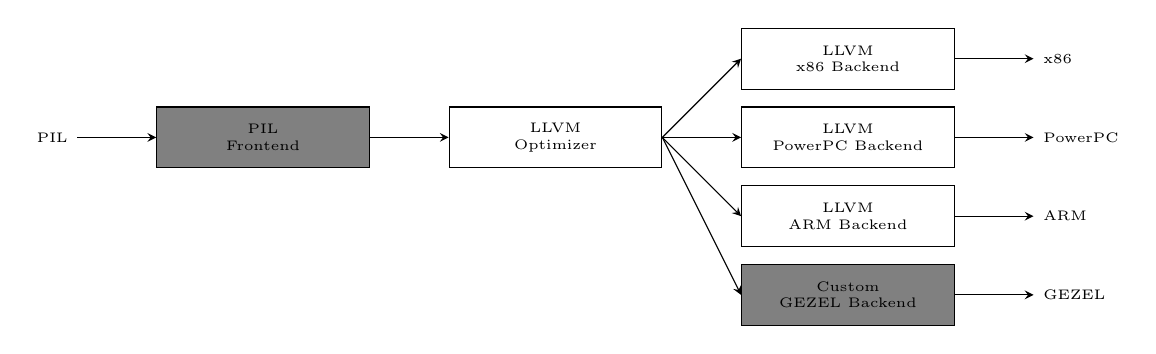
\begin{tikzpicture}[>=stealth]
    \tikzstyle{lang}=[rectangle,draw=black,thin,font=\tiny,inner
    sep=0pt, align=center,minimum width=2.7cm,minimum height=2.2em]

    \tikzstyle{txt}=[font=\tiny]

    \node[lang](llvm_opt){LLVM \\ Optimizer};
    \node[lang](ppc_back)[right=1 cm of llvm_opt]{LLVM \\ PowerPC Backend};
    \node[txt](ppc)[right=of ppc_back]{PowerPC};
    \node[lang](x86_back)[above of=ppc_back]{LLVM \\ x86 Backend};
    \node[txt](x86)[right=of x86_back]{x86};
    \node[lang](arm_back)[below of=ppc_back]{LLVM \\ ARM Backend};
    \node[txt](arm)[right=of arm_back]{ARM};
    \node[lang,added](gezel_back)[below of=arm_back]{Custom \\ GEZEL Backend};
    \node[txt](gezel)[right=of gezel_back]{GEZEL};

    \node[lang,added](pil_front)[left=1 cm of llvm_opt]{PIL \\ Frontend};
    \node[txt](pil)[left=of pil_front]{PIL};

    \draw[->] (pil_front.east) -- (llvm_opt.west);

    \draw[->] (llvm_opt.east) -- (x86_back.west);
    \draw[->] (llvm_opt.east) -- (ppc_back.west);
    \draw[->] (llvm_opt.east) -- (arm_back.west);

    \draw[->] (x86_back) -- (x86);
    \draw[->] (ppc_back) -- (ppc);
    \draw[->] (arm_back) -- (arm);

    \draw[->] (pil) -- (pil_front);

    \draw[->] (llvm_opt.east) -- (gezel_back.west);

    \draw[->] (gezel_back) -- (gezel);
  \end{tikzpicture}
  \caption{LLVM custom workflow (changes highlighted)}
  \label{fig:custom_llvm_workflow}
\end{figure}

\newpage

\subsection{Extensions to PIL}
\label{subsec:pil_extensions}

\subsubsection{Multiple Blocks}

The base PIL language supported only a Prover and a Verifier block
besides the Common block. This makes it impossible to implement a
multiparty protocol\footnote{In the cryptographic world, this means
  three or more parties}. As this is simply a relaxation of the rules,
the change to the grammar and the code generator was trivial.

\subsubsection{Compile Time/Constant Expressions}

Compile time/constant expressions were needed to allow more advanced
specifications of protocols. The PIL language does not specify
constant expressions as parameters of variables. When designing more
complex protocols where parameters of variables have to be adjusted,
one needs constant expressions. The benefit of constant expressions
can be seen from the following example:
\begin{lstlisting}[language=PIL]
Common (
  Z l_n = 1024;
  Z l_f = 160;
  Z l_e = 410;
  Z l_e_1 = 120;
  Z l_v = 1512;
  Z l_phi = 80;
  Z l_H = 160;
  Prime(l_n) n = 17
) {

}

Smartcard (
  Zmod*(n) p, q;
  Int(l_f + l_phi + l_H) f
) {
  Zmod*(n) S, _Z, R;
  Int(l_n + l_phi) v_1;
  Int(l_v) v;
  ...
\end{lstlisting}
Without constant expressions, one would need to recompute the values
manually and enter them every time a change was desired. This
re-computation and reentering is prone to errors and as such
undesirable when designing a crypto framework. The grammar change to
allow constant expressions is very simple
\begin{lstlisting}[language=grammar, keywords={group, expr}]
group	:	('Zmod+'|'Zmod*') '(' expr ')' 
	|	'Prime' '(' expr ')'
	|	'Int' '(' expr ')'
	|	'Z'
	;
\end{lstlisting}
This change allows it only syntactically so some semantic processing
will be needed to ensure that they are constant expressions which can
be evaluated at compile time by the compiler.

\subsubsection{Type Inference}

To be able to check for correctness, one needs to determine the resulting
type of a certain expression. This can be also used to allow one to omit
a type declaration. The following example illustrates this:
\begin{lstlisting}[language=PIL]
Zmod*(p) b;
x := Random(Int(80));
a := b^x;
\end{lstlisting}
For the case of variable x, its type can be inferred as Int(80) since
the Random function can only return a random value of the provided
type. For the case of variable a, the situation is a bit more
complex. However, if the operation of exponentiation is defined as
applying the multiplication operation many times, then the type of a
can only be Zmod*(p) by the definition of the multiplicative modular
residue group. A similar case can be made when multiplying an element
of the additive modular residue group with an integer. This means that
the type inference is well defined for any acceptable operation in
PIL.

\section{PIL Front-end}
\label{sec:pil_frontend}

PIL frontend flow is depicted in Figure \ref{fig:pil_frontend_flow}.  An
input PIL is read by the Lexer producing input for the Parser. The
Parser reads these and generates an abstract syntax tree (AST) which
is fed to the Codegen tree-walker that generates the code (in the form
of LLVM IR). Both the lexer grammar and the parser grammar are
specified in the file pil.g. The tree-walker and the code generator is
specified in the file codegen.g.

\begin{figure}[hb!]
  \centering
  \subfloat{
  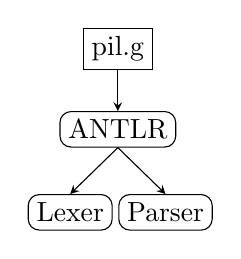
\begin{tikzpicture}[>=stealth]
    \tikzstyle{edge from parent}=[draw,->]

    \Tree[.\node[language](parser_g){pil.g};
      [.\node[compiler](antlr){ANTLR};
        [.\node[compiler](lexer){Lexer};]
        [.\node[compiler](parser){Parser};]
      ]
    ]
  \end{tikzpicture}
  } \qquad
  \subfloat{
  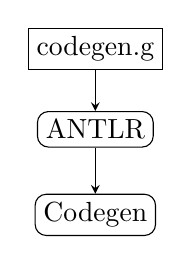
\begin{tikzpicture}[>=stealth]
    \tikzstyle{edge from parent}=[draw,->]

    \Tree[.\node[language](tree_g){codegen.g};
      [.\node[compiler](antlr2){ANTLR};
        [.\node[compiler](walker){Codegen};]
      ]
    ]
  \end{tikzpicture}
  }
  \caption{Lexer, parser and tree walker generation}
\end{figure}

\begin{figure}[hb!]  
  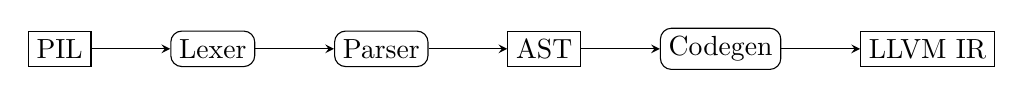
\begin{tikzpicture}[>=stealth]
    \node[language] (pil) {PIL};
    \node[compiler] (lexer) [right=of pil] {Lexer};
    \node[compiler] (parser) [right=of lexer] {Parser};
    \node[language] (ast) [right=of parser] {AST};
    \node[compiler] (codegen) [right=of ast] {Codegen};
    \node[language] (llvm_ir) [right=of codegen] {LLVM IR};

    \draw[->] (pil) -- (lexer);
    \draw[->] (lexer) -- (parser);
    \draw[->] (parser) -- (ast);
    \draw[->] (ast) -- (codegen);
    \draw[->] (codegen) -- (llvm_ir);
  \end{tikzpicture}
  \caption{PIL frontend flow}
  \label{fig:pil_frontend_flow}
\end{figure}

The code generation process generates one module per block. The Common
block module is augmented with the functions provided by the VM.
Every other block except the Common block gets a Common block linked
in. This process is depicted in Figure \ref{fig:linker}.

\begin{figure}[hb!]
  \centering
  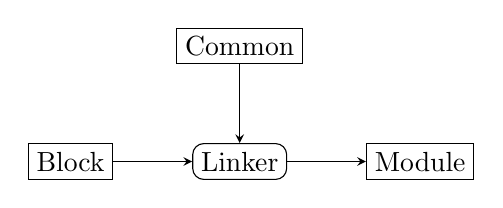
\begin{tikzpicture}[>=stealth]
    \node[language] (block) {Block};
    \node[compiler] (linker) [right=of block] {Linker};
    \node[language] (common) [above=of linker] {Common};
    \node[language] (module) [right=of linker] {Module};

    \draw[->] (block) -- (linker);
    \draw[->] (common) -- (linker);
    \draw[->] (linker) -- (module);
  \end{tikzpicture}
  \caption{Linker}
  \label{fig:linker}
\end{figure}

The private parameters as well as global variables are transformed as
LLVM IR global variables, the private parameters being constant in
this case. Each function of a block gets transformed as an LLVM IR
function with its input and output arguments transformed as such. LLVM
allows for multiple return values so this is used as well when there
are multiple return values.

LLVM's constant folder is used to evaluate constant time expressions
to simplify them into a constant value.

When dealing with group arithmetic, which LLVM does not support, there are
two possibilities:
\begin{enumerate}
\item extend the LLVM's type system to include group types - this
  involves editing the core LLVM files, adding a new DerivedType,
  changing the bit-code format and adding changes to the LLVM parser
  (both binary and textual). Also, binary operations have to be redefined
  to support these new types \cite{extending_llvm}.
\item use a simpler, existing LLVM type and make the compiler do the
  extra work - the IntegerType of LLVM can be used for arbitrarily sized
  integers.
\end{enumerate}

The first option allows for preserving the information about the
modular residue groups to the lowest level. The transformation to a
primitive type supported by the target architecture happens only at a
later stage. Or, if the target architecture supports modular residue
groups, there is no need for a transformation, only a translation.
This allows for a code that is more verifiable and more secure as the
properties are kept to the lowest possible levels (no exploits can be
made under secure starting conditions). The disadvantage of this
method is the changes that need to be introduced at the heart of such
a complex framework as LLVM is. This is both time consuming and error
prone. Also, it becomes more difficult to track newer versions of LLVM
(with possibly better optimizations and more features) if the changes
are not integrated back into the main project. This method also breaks
compatibility with existing LLVM applications, so a specially patched
version of LLVM needs to be distributed.

The second option is easier as the changes to the compiler are only
local and do not break compatibility with existing LLVM applications.
It is also easier as there is no hard work associated with changing
the core of LLVM. More work has to be assigned to the compiler because
it needs to track types and apply the appropriate operations in the
case of modular residue groups. The burden is also on the back-end if
an architecture supports modular residue groups since it now has to
regenerate the lost information. An example of such an architecture
can be an automatic verifier whose job is now made more complex. This
re-generation of information might also not be always completely
accurate.

The first approach was attempted first but was deemed too time
consuming and error prone. Also it would require some standardization
with LLVM upstream to allow future tracking. The second approach was
chosen as the one to base the work on. The types are backed by an
IntegerType of the appropriate length in the LLVM IR. Type inference
was used to deduce the resulting type of an operation. The operation
was then sent to appropriate 3 argument operations with the first 2
being the operands as integers and the third operand being the
modulus.

\subsection{Type Alias}

Type aliases are evaluated and substituted by the parser. The
reasoning behind them can go both ways. Although they are more
semantic than syntactic since they convey information (as a creation
of another type), they are simple enough to be evaluated and
substituted by the parser. This can be paralleled with a pre-processor
in languages which support it. The rule includes a syntactic predicate
to test if it is a declaration of an alias or an alias is referenced.
\begin{lstlisting}[language=C++, keywords={ID, group, interval, alias}]
alias :
      (ID '=' )=> ID! '='! (
        group { aliases[(const char*)$ID.text->chars] = $group.tree; } 
      | interval { aliases[(const char*)$ID.text->chars] = $interval.tree; }
      )
      |	ID -> { aliases[(const char*)$ID.text->chars] }
      ;
\end{lstlisting}
If the syntactic predicate matches, the alias is stored in a hashmap,
otherwise the hashmap is searched for the alias. This syntactic
predicate effectively implements a 1 symbol look-ahead.

\subsection{Type system}

The compiler has to keep track of the types. A simple type system was
designed that allows both numbers and modular residues. The UML of
this type system is given in Figure \ref{fig:type_system}.

\begin{figure}[hb!]
  \centering
  \begin{tikzpicture}
    \tikzumlset{font=\tiny}

    \umlclass{NumberT}{
      \# width : const uint64\_t
    }{
      \umlvirt{+ getType() : llvm::Type} \\ 
      \umlvirt{+ getBitWidth() : uint64\_t}
    }
    \umlclass[y=-3]{GroupT}{
      \# modulus : const llvm::APInt
    }{
      + getModulus() : llvm::APInt \\
      + getModulusConstant() : llvm::ConstantInt
    }
    \umlinherit{NumberT}{GroupT}
  \end{tikzpicture}
  \caption{Type system UML}
  \label{fig:type_system}
\end{figure}

NumberT represents any general number type that can occur (types Int
and Z), while GroupT represents group types (types Zmod+ and Zmod*). The
getType() method returns the backing type in the LLVM IR (IntegerType
of the appropriate length). The modulus of the GroupT is stored as an
LLVM arbitrary precision integer (llvm::APInt) and it can be fetched
by using the getter getModulus(). getModulusConstant() is a helper
method that wraps it in a ConstantInt which LLVM can then use for
constant folding.

\subsection{Type Inference}

The easiest approach for determining a resulting type from two
operands is to use double dispatch and code each of the resulting
functions.  There were some attempts at bringing multiple dispatch to
C++ but this has still not been realized \cite{c++_multi_methods}.

A common way to simulate it in C++ is to use a visitor pattern. The
base interface or the base class defines accept methods. The visitor
then calls each of the classes dispatching itself as a parameter. Here
is how it is done with GroupT and NumberT:

\begin{lstlisting}[language=C++]
class NumberT {
  ...
  virtual NumberT *addWithSubFrom(const NumberT *first);
  ...
  virtual NumberT *operator+(const NumberT &other) const {
    return other.addWithSubFrom(this);
  }
};

class GroupT : public NumberT {
  ...
};
\end{lstlisting}

Here the addWithSubFrom method is the accept method.  The same was
done for each of the operators. When the compiler encouters a + b
where a and b have NumberT as a base class, it will call the
\textbf{operator+}. This call happens through a \emph{vtable} so the
\emph{this} pointer always points to the accurate type for the first
operand. By calling the addWithSubFrom method, another \emph{vtable}
dispatch happens and withing the addWithSubFrom \textbf{this} points
to the accurate type for the second operand \cite{Eckel}. Since both
of the operands are now correctly resolved it remains to return the
resulting type of the operation. Extending the type inference simply
involves writing a function for each combination of the operand
types. This is somewhat easier than using Run Time Type Information
and writing an if-then-else or similar for each of the cases.

Since GroupT derives from NumberT the operator calls will remain this
way unless overridden. The accept methods will need to be overridden
as they provide the custom logic for each of the combinations.

The classes NumberT and GroupT also define methods for creating an
LLVM instruction for addition, subtraction, multiplication and
exponentiation. These function as adapters and make the process of
code-generation uniform. Here is an excerpt from the code generation:
\begin{lstlisting}[language=C++, morekeywords=expr]
expr[const char *id] returns [Value *value, NumberT *type]
	:	...
	|	^('+' lhs=expr[$id] rhs=expr[$id]) {
                  $type = *$lhs.type + *$rhs.type;
                  $value = $type->createAdd($lhs.value, $rhs.value);
                }
	|	...
\end{lstlisting}

\section{GEZEL Back-end}

The GEZEL Back-end extracts the Data Flow Graph (DFG) and implements
one GEZEL datapath per round (Figure \ref{fig:gezel_backend}). The
Control Flow Graph (CFG) is maximally unrolled such that the DFG
within a round is purely combinatorial. Each invocation of addition,
multiplication, exponentiation requires a new instantiation of an
adder, multiplier, exponentiator, respectively.


\begin{figure}[hb!]
  \centering
  \begin{tikzpicture}[>=stealth]
    \node[language, inner sep=0.5cm](round0){Round0};
    \node[language, inner sep=0.5cm](round1)[below=of round0]{Round1};
    \node[language, inner sep=0.5cm](round2)[below=of round1]{Round2};

    \node[language, inner sep=0.5cm](regs)[above=of round0]{Registers};

    \node[language, inner sep=0.5cm](mux_in)[left=2cm of round1]{Input bus};

    \node[language, inner sep=0.5cm](mux_out)[right=2cm of round1]{Output multiplexer};

    \draw[->](round0.east) -- (mux_out.west);
    \draw[->](round1.east) -- (mux_out.west);
    \draw[->](round2.east) -- (mux_out.west);
    \draw[->](mux_in.east) -- (round0.west);
    \draw[->](mux_in.east) -- (round1.west);
    \draw[->](mux_in.east) -- (round2.west);
    \draw[->](regs.west) -- (mux_in.north |- regs.west) -- (mux_in.north);
    \draw[->](mux_out.north) -- (mux_out.north |- regs.east) -- (regs.east);
  \end{tikzpicture}
  \caption{Generated GEZEL model of Schnorr's protocol}
  \label{fig:gezel_backend}
\end{figure}

The choice of maximally unrolling the CFG was made as it already
allows architecture exploration at one end of the spectrum while the
other is provided by the software implementation. The implementations
in the middle of the spectrum should be derived from the closer side
by rolling the CFG or adding more to the software. Such techniques
require more complex signaling and scheduling and, as time was
limited, were not taken.

The memory accesses are converted to register accesses and each
datapath gets access to each of the registers. To prevent name collisions
register inputs and outputs are decorated as shown below:

\filbreak

\begin{lstlisting}[language=GEZEL]
dp round1(in  r_r_1_i : ns(160); out r_r_1_o : ns(160);
          in  r_s_1_i : ns(160); out r_s_1_o : ns(160);
          out _t_1 : ns(1024)) {
          
  sig s_r_1 : ns(1024);
  sig s_t_1 : ns(1024);

  use random1(11, s_r_1);
  use modexp1(3, s_r_1, 23, s_t_1);
  
  always {
    r_r_1_o = s_r_1;
    r_s_1_o = r_s_1_i;

    _t_1 = s_t_1;
  }
}
\end{lstlisting}

The example is generated from the Schnorr's Identification Protocol
PIL (see example of \ref{subsec:pil}). Each register is prefixed with
\emph{r} and suffixed with \emph{i} if referring to the input from the
register or \emph{o} if referring to the output from the register. The
internal signals within a datapath are prefixed with \emph{s}.

%%% Local Variables: 
%%% TeX-PDF-mode: t
%%% TeX-master: "thesis"
%%% End: 


%-	If submission is not anonymous think on making a web-page to upload the source code, and explain how to compile, execute and configure it.
%-	Describe implementation
%-	Describe efficiency and (possibly) compare it

%%% Local Variables: 
%%% TeX-PDF-mode: t
%%% TeX-master: "main"
%%% End: 


\chapter{Conclusion}

%%% Local Variables: 
%%% TeX-PDF-mode: t
%%% TeX-master: "thesis"
%%% End: 


\printbibliography

\end{document}

%%% Local Variables: 
%%% TeX-PDF-mode: t
%%% TeX-master: t
%%% End: 
